%% FONT SIZE REFERENCE

%% \tiny sample text
%% \scriptsize sample text
%% \footnotesize sample text
%% \small sample text
%% \normalsize sample text
%% \large sample text
%% \Large sample text
%% \LARGE sample text
%% \huge sample text
%% \Huge sample text

% document class:
\documentclass[10pt]{article}

%% \usepackage{subfigure} % for subfigures
\usepackage{amsmath}
\usepackage{amssymb} % for math symbols
\usepackage{graphicx} % image formats
\usepackage[top=2cm,bottom=2cm,left=2cm,right=2cm]{geometry} % define page set up
\usepackage{float}
\usepackage{listings}
%% \usepackage{columbidaeTitle}
%% \usepackage{dirtree}
\usepackage[normalem]{ulem}
\usepackage{lscape}
\usepackage{csvsimple}
\usepackage{multicol}
\usepackage{caption}
\usepackage{subcaption}

%% \usepackage{titlesec}

\usepackage{makecell}

\renewcommand\theadalign{bc}
\renewcommand\theadfont{\bfseries}
\renewcommand\theadgape{\Gape[0pt]}
\renewcommand\cellgape{\Gape[0pt]}


\setcounter{secnumdepth}{3}

%% \titleformat{\paragraph}
%%             {\normalfont\small\bfseries}{\theparagraph}{1em}{}
%%             \titlespacing*{\paragraph}
%%             {0pt}{3.25ex plus 1ex minus .2ex}{1.5ex plus .2ex}

%% \titleformat{\section}[hang]{\normalfont\Large\bfseries}{\thesection:\ }{0.5ex}{}
%% \titleformat{\subsection}[hang]{\normalfont\large\bfseries}{\thesubsection:\ }{0.5ex}{}
%% \titleformat{\subsubsection}[hang]{\normalfont\normalsize\bfseries}{\thesubsubsection:\ }{0.5ex}{}
            
            
\newcommand{\hin}{\hangindent=8mm \hangafter=1 \noindent }

% color package:
\usepackage{color}
\newcommand{\edit}{\textcolor{red}} % marker to designate areas that need future attention
\newcommand{\neal}{\textcolor{blue}} % marker to designate neal action item

\newcommand{\teurer}{\textbf\Large}
\newcommand{\teuer}{\textit}

\definecolor{passgreen}{rgb}{0,0.5,0}
\definecolor{failred}{rgb}{0.5,0,0}

%% \newcommand{\tableheader}{\textbf}
\newcommand{\subtitleaccent}{\textsuperscript{\line(1,0){40}}}
%% \newcommand{\usecase}{\large\underline}
%% \newcommand{\testscenario}{\normalsize}
%% \newcommand{\testcase}{\small\textit}
%% \newcommand{\passtest}{\textcolor{passgreen}}
%% \newcommand{\failtest}{\textcolor{failred}}

\usepackage{setspace}
%% \doublespacing
\singlespacing

% set to zero indent length
\setlength\parindent{0pt}

\definecolor{mygray}{rgb}{0.98,0.98,0.98}
\lstset{ %
  backgroundcolor=\color{mygray},
  frame=single
}

%% \newenvironment{changemargin}[2]{%
%%   \begin{list}{}{%
%%       \setlength{\topsep}{0pt}%
%%       \setlength{\leftmargin}{#1}%
%%       \setlength{\rightmargin}{#2}%
%%       \setlength{\listparindent}{\parindent}%
%%       \setlength{\itemindent}{\parindent}%
%%       \setlength{\parsep}{\parskip}%
%%     }%
%%   \item[]}{\end{list}}

%% \DTsetlength{0.2em}{3em}{0.2em}{0.4pt}{1.6pt}

\title{%
  The Consumer Coffee Maker \\
  {\large \subtitleaccent~~Purchasing and Design Heuristics through Modeling and Simulation~~\subtitleaccent}}
%% \project{HydroClient 1.4.1}
\author{%
  ~\\
  Neal DeBuhr and Andre Baptiste\\
  ~\\
  School of Computing, Informatics, and Decision Systems Engineering\\
  Arizona State University, Tempe, AZ, USA, 85281
}
\date{\today}

\begin{document}

\maketitle

\newpage
\tableofcontents
\newpage

\section{Introduction}
\label{sec:int}
Globally, annual coffee production last year was 9 million metric tons (Coffee market...) - this is equivalent to about a million African elephants (Frei) in weight, and fills 150 million 60 kg coffee sacks. Coffee is clearly loved around the world. For some, the drink is an experience - a treat to be enjoyed when a suitable occasion arises. For others, coffee is a necessary foundation of a productive day of work and activity. Regardless of the reasons for drinking, very few people understand the mechanics of coffee brewing. This is evident by uninformed consumer decisions regarding coffee makers. Despite an appearance of simplicity, coffee makers can be understood through a wide variety of experimental frames, levels of system specification, and modeling paradigms. Through modeling and simulation, valuable insights about coffee brewing can be uncovered.

\subsection{Experimental Frames}
The system can be framed from the hydrological/chemical perspective, thermodynamic perspective, control systems perspective, or the user perspective (to name just a few). The experimental frame serves as a lens for any modeling and simulation effort. For this report, the system will be approached primarily in a thermodynamic and control systems experimental frame. Using this frame enables the capturing of core user IO behavior, as well as the fundamental coffee brewing thermodynamic behavior. Other possible experimental frames will be largely reduced to assumptions. For example, the fluid mechanics will be reduced to an assumption of constant mass flow rate between the boiler and coffee pot during brewing. Further, the chemical composition of the water will be treated as a parameter, rather than a variable.

\subsection{Levels of System Specification}
There is value in developing multiple specifications of the model, at varying levels of specification.  However, the ``coupled component'' (level four) system specification (Zeigler) will serve as the primary lens on the system during analysis.  This level of specification combines component systems through IO behavior, and is particularly intuitive/meaningful for the coffee maker system.  A representation of the system is provided in Figure \ref{fig:sysSpeDia}.  %With rigorously defined system structure and behavior, this representation is a level four system specification.

\begin{center}
  \begin{figure}[H]
    \begin{subfigure}{.5\textwidth}
      \centering
      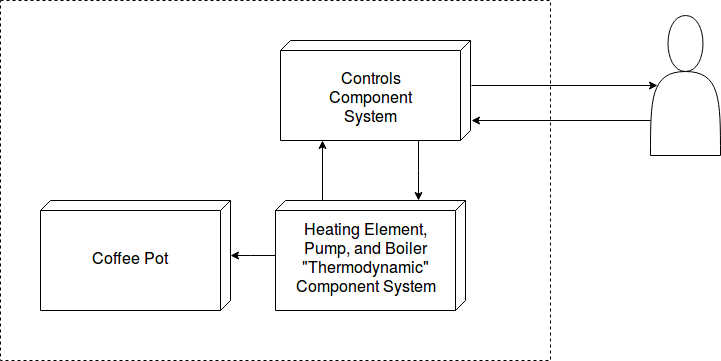
\includegraphics[width=.8\linewidth]{input/Decomposed_v04}
      \caption{Coupled Decomposed System Diagram}
      \label{fig:sysSpeDia}
    \end{subfigure}%
    \begin{subfigure}{.5\textwidth}
      \centering
      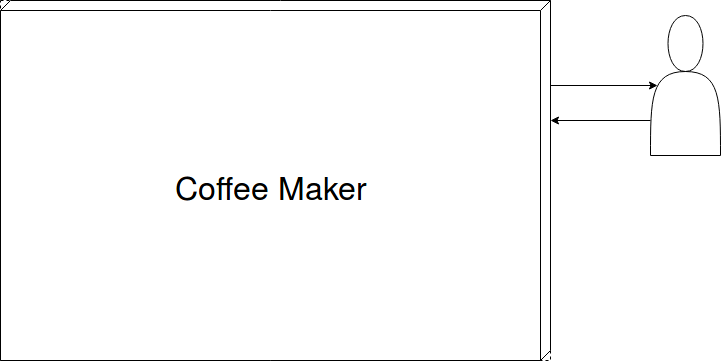
\includegraphics[width=.8\linewidth]{input/Composed_v04}
      \caption{Atomic Composed System Diagram}
      \label{fig:comSysDia}
    \end{subfigure}
  \caption{System Diagrams at Different Levels of Decomposition}
  \end{figure}
\end{center}

Presenting these components as a larger system provides an alternative perspective on the system (Figure \ref{fig:comSysDia}).  This in turn lends itself to analysis of the behavioral, as opposed to structural, dynamics of the system. In the sense that this representation of the system does not capture structure and component system coupling, it is a lower level system specification (level three).  However, being that the composed model exhibits closure under coupling, the same tools for analysis of the atomic component models can be used to analyze the composed model.  This presents opportunities for additional insight and analytical flexibility for the modeling and simulation effort.

System inference and system design are outside the scope of this project.  Rather, this project takes a systems analysis perspective on modeling and simulation.  As such, the foundational model for this project is a high level system specification.  From there, lower level system specifications are generated and interpreted.

%% \subsection{Taxonomy}
%% The flexibility of coffee maker simulations enables a wide variety of valuable analysis.  However, simulation of the human agent provides little value, given the experimental frame and objective of the project.  Instead, real people will interact with the system.  This approach offers flexibility, a valuable dose of spontaneity, and a smaller gap between simulation and reality.  The taxonomy described here can be referred to as Virtual Simulation - a type of taxonomy introduced by the Defense Modeling and Simulation Organization (Sarjoughian, Modeling Concepts...).

\subsection{Modeling Formalism}
\label{sec:modPar}
Most modern coffee makers utilize digital, discrete-time systems for measurement, control, and interacting with the user.  However, the underlying thermodynamic, chemical, and electromechanical behavior lends itself to continuous-time representation.  This plurality of possible time bases, along with a multitude of formats for quantifying input, state, and output (eg. ``dispensing'' vs. +13 mL/sec), gives rise to a great number of modeling formalism possibilities.  In this project, the discrete event system specification (DEVS) formalism is used for simulation.  This modeling paradigm captures the system dynamics of the control system with relative ease.  However, the thermodynamic behavior is a bit more difficult to capture with this modeling formalism.  The boiler heating element, pump, and coffee pot fluid mixing would most naturally be quantified through a differential equation system specification.  However, by discretizing the differential equations (more details on this in Section \ref{sec:buiTheSysSpe}), a discrete time system specification arises.  This way, the ``DEVS Wrapper'' approach can be employed to simulate the discrete time behavior within a DEVS environment.  The DEVS Bus approach brings power and flexibility to the modeling effort, mainly due to the ``universality of the DEVS representation and the ability of DEVS bus to support the basic system formalisms'' (Zeigler).  The only externality of the formalism embedding described above is the creation of a ``time step'' parameter.  With smaller values for the time step parameter, the DEVS simulation results will converge with the differential equation system specification behavior.  For this modeling project, the DEVS Suite software will serve as the simulator for the DEVS modeling described above.


% COuld talk about quantization (page 9 main textbook) here.

%% \subsection{System Specification Morphisms}
%% Morphism is about relating models/simulators/etc. at the same level of system specification.  Only one model is within scope for this modeling initiative.  As such, there is not much to comment on as far as system morphism. 

\section{System Classification}
The coffee maker system being modeled is in some sense a cyber-physical system.  Cyber-physical systems
\begin{quote}
``combine computing and networking with physical dynamics. Cyber-physical systems require model combinations that integrate the continuous dynamics of physical processes (often described using differential equations) with models of software.  Diverse models are most useful in applications where timed interactions between components are combined with conventional algorithmic computations,'' (Ptolemaeus).
\end{quote}
While networking details are not considered in this analysis, this system classification is otherwise fitting.  Cyber-physical systems are often at the heart of modeling and simulation activities.  As such, the modeling and simulation insights generated by this project may be adaptable to a wide variety of other interesting systems.  

\section{Problem Description}

\subsection{Questions}
This report approaches the coffee maker system from the thermodynamic and electronic perspective.  Valuable and actionable insights is the objective of the modeling and simulation effort.  Providing coffee consumers with additional insight into the coffee brewing process will relieve some of the information asymmetry in the market - a key problem detailed in Section \ref{sec:int}.  While a holistic and open-minded perspective is applied to the interpretation of the simulation results, some possible questions addressed by the modeling and simulation effort include:
\begin{itemize}
\item How does the selection of thermodynamic components influence the behavior of the brewer?
\item Does the controls system latency give rise to any instability, or otherwise problematic behavior?
\item What issues arise at the intersection of the digital control system electronics and the analog electromechanical system?
\item How does erroneous user behavior impact coffee maker performance?
\item Do stability and/or safety issues arise for simple heating systems and simple safety shutoff systems?
\end{itemize}

\subsection{Assumptions}
\label{sec:ass}

The following assumptions support a simplification of the problem and a focus on the desired experimental frame:
\begin{itemize}
\item Constant mass flow rate during coffee pot filling
\item Perfectly insulated boiler and coffee pot - no convection or conduction heat loss
\item Absence of any radiative heat transfer
\item Constant thermodynamic properties\footnote{While thermodynamic properties can vary by temperature and pressure, the change is relatively small for environments close to room temperature and sea level pressure - these relatively small changes can be ignored with negligible impact on results}
\item No mass loss through steam or other mechanisms
\item Ideal operation of boiler heating element - constant heat flux
\item Complete absence of impurities in water - water is considered distilled
\item No consideration for chemical reactions between the water and brewer components (e.g. rusting)
\end{itemize}

\section{Approach}
\subsection{Model Development}
The essential construct of the system includes a boiler system component model, a coffee pot component model, and modeled digital electronics for user interaction and coffee maker control.  The system is open with respect to defined user inputs (eg. user pressing the ``On'' button) and outputs (eg. indicator lights to inform the user of brewing state).
%To understand the construction of the model and behavior of the component systems, a qualitative IOFO specification is considered, followed by a system diagram, and then mathematical characterization of key inputs, outputs, and functions.


%% For the thermodynamic system, the a list of high-level states include:
%% \begin{itemize}
%% \item Off (Cooling)
%% \item Heating
%% \item Maintain Temperature
%% \end{itemize}

%% For the user interface and control system, the list of high-level states include:
%% \begin{itemize}
%%   \item Standby
%%   \item Brewing
%%   \item Warming
%%   \item Shutdown
%% \end{itemize}

\subsubsection{System Diagram}
\begin{center}
  \begin{figure}[H]
    \begin{center}
      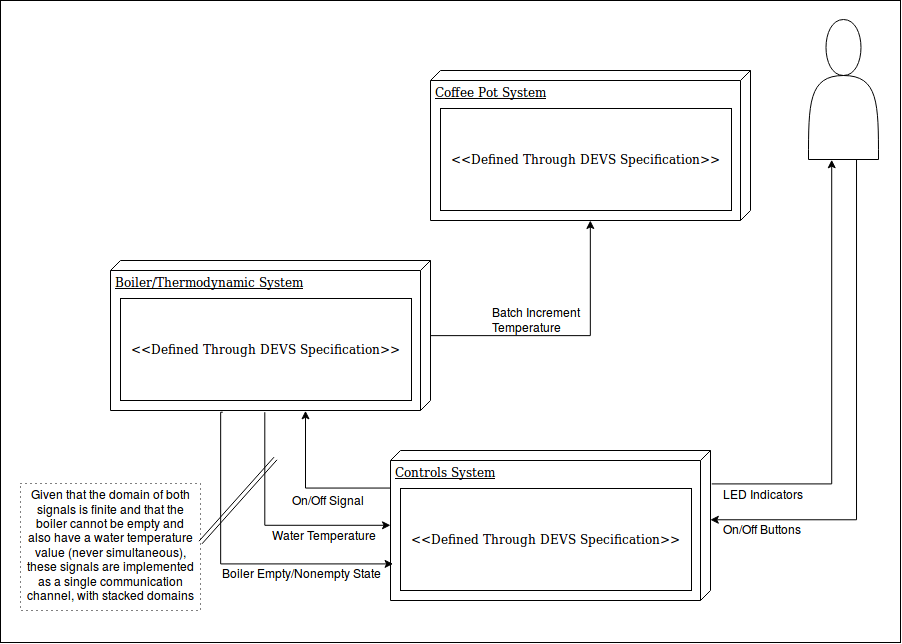
\includegraphics[width=0.9\textwidth]{input/Coffee_Maker_v05}
      \caption{System Diagram for Coffee Maker Model and Simulator}
      \label{ref:sysDia}
    \end{center}
  \end{figure}
\end{center}

\subsection{System Specification}
Given that this project is a systems analysis initiative, the foundational definition of the system is a high level system specification.  As the analysis proceeds, lower level system specifications are produced.

\begin{figure}[H]
\begin{center}
\begin{tabular}{c}
  \fbox{I/O System} \\
  $\downarrow$ \\
  \fbox{I/O Function Observation} \\
  $\downarrow$ \\
  \fbox{I/O Relation Observation} \\
  $\downarrow$ \\
  \fbox{I/O Observation} \\
\end{tabular}
\end{center}
\caption{System Specification Hierarchy}
\label{fig:sysSpeHei}
\end{figure}

%% Having knowledge of the system structure allows us to deduce, through analysis and simulation, the system behavior (the outer manifestation of the system).

%% Given the heirarchal nature of system specifications, lower level specifications can be generated more or less procedurally.  Working down the levels makes information which is implicit at higher system specification levels explicit.  While there can be some value in deducing lower level specifications from higher level ones, there isn't any new information introduced by the process.  As such, instead of starting from the highest level of system specification, this section details an incremental approach to development of the top level specifications.  From the observation frame (lowest level specification) to the coupled system specification (highest level considered here), the system specification is continually developed, expanded, and refined.  This is not to be interpreted as generating a high level information from a low level specification, as would be seen in systems inference and systems design approaches.  Rather, the levels of specification provide a convinient way to incrementally develop the perspectives and details of a high level specification.


%% \subsubsection{Observation Frame}
%% While the observation frame is often considered the foundational level of system specification, it is not subject to the same degree of mathematical formality.  From \edit{Citation here}, ``the Observation Frame specifies how to stimulate the system with inputs:
%% what variables to measure and how to observe them over a time base.''.  In fact, the experimental frame and I/O port choices are implicitly detailed in much of the previous sections.  Nevertheless, a more explicit discusssion of these details follows.

%% \paragraph{Foundational Definitions and Considerations}
%% Being a dynamic system, the passage of time is central to a successful modeling of the coffee maker system.  We define time as:
%% \begin{center}
%% \begin{tabular}{r c l}
%%   time & = & (T, $<$) \\
%% \end{tabular}
%% \end{center}
%% T is a set of time values which cannot be established apriori.  Rather, we allow events to happen at any time such that:

%% $T = \{~t~\epsilon~T~|~t~\epsilon~\mathbb{R}~\}$

%% The ordering for the coffee maker is linear, or total, in that we can relate any pairs of time values with $<$, $>$, or $=$.  Through the use of the DEVS-Suite simulator in a non-distributed setting, this is naturally the case.

\subsubsection{Model Components Qualitative Description}

Thinking about the system holistically is an important predecessor to a more rigorous mathematical definition.  As such, this section seeks to provide some context and focus for component system structure and behavior.  Of particular importance is considering how the component systems will interact, and ports/constructs by which the system structure translates to system behavior.
\begin{figure}[H]
\fbox{\begin{minipage}{0.98\textwidth}
\textbf{Thermodynamic Component System} \\
\teuer{Quantized DESS Embedded in DEVS} \\
\teuer{Signals are Discrete Events} \\

\vspace{0.2cm}

\begin{minipage}{0.48\textwidth}
\begin{small}
\begin{itemize}
\item Input
  \begin{itemize}
  \item Brew Signal - Coupled with Controls System
  \item Off Signal - Coupled with Controls System
  \end{itemize}
\item Output
  \begin{itemize}
  \item Water Temperature - Coupled with Controls System
  \item Boiler Emptiness - Coupled with Controls System
  \item Incremental Brew Volume - Coupled with Coffee Pot System
  \end{itemize}
\item Functions
  \begin{itemize}
  \item Heat Flux - Internal State Transition
  \item Brewing Flow - Internal State Transition
  \item Brew Initiation - External State Transition
  \item Brew Termination - External State Transition
  \end{itemize}
\end{itemize}
\end{small}
\vfill
\end{minipage}%
\begin{minipage}{0.04\textwidth}
  ~\\
\end{minipage}%
\begin{minipage}{0.48\textwidth}
  \begin{small}
    \begin{itemize}
\item Parameters
  \begin{itemize}
  \item Water Volume
  \item Heating Element Power
  \item Specific Heat Capacity of Water
  \item Fluid Density
  \end{itemize}
\item State Variables
  \begin{itemize}
  \item Boiler Phase
  \item Boiler Water Temperature
  \item Fluid Portion in Pot
  \item Time Until Next Event ($\sigma$)
  \end{itemize}
\end{itemize}
\end{small}
\vfill
\end{minipage}
\end{minipage}}
\caption{Thermodynamic System Interfaces and Qualitative Structure}
\label{fig:IOFO1}
\end{figure}

\vspace{0.2cm}

\begin{figure}[H]
\fbox{\begin{minipage}{0.98\textwidth}
\textbf{Controls Component System} \\
\teuer{DEVS} \\
\teuer{Signals are Discrete Events} \\

\vspace{0.2cm}

\begin{minipage}{0.48\textwidth}
\begin{small}
\begin{itemize}
\item Input
  \begin{itemize}
  \item On/Off Buttons - Inputs from User
  \item Water Temperature - Coupled with Thermodynamic System
  \item Boiler Emptiness - Coupled with Thermodynamic System
  \end{itemize}
\item Output
  \begin{itemize}
  \item User LED Indicators - External Output to the User
  \item Brew Signal - Coupled with Thermodynamic System
  \item Off Signal - Coupled with Thermodynamic System
  \end{itemize}
\end{itemize}
\end{small}
\vfill
\end{minipage}%
\begin{minipage}{0.04\textwidth}
  ~\\
\end{minipage}%
\begin{minipage}{0.48\textwidth}
  \begin{small}
    \begin{itemize}
\item Functions
  \begin{itemize}
  \item User Commands - External State Transition
  \item Temperature Safety Shutoff - External State Transition
  \item Brew Completed Shutoff - External State Transition
  \item Safety Timeout - Internal State Transition
  \item Indicators Timeout - Internal State Transition
  \end{itemize}
%% \item Function - (potentially) timer/scheduled-brew datetime functions
\item State Variables
  \begin{itemize}
  \item Controls Phase
  \item Time Until Next Event ($\sigma$)
  \end{itemize}
\end{itemize}
\end{small}
  \vfill
  \end{minipage}
\end{minipage}}
\caption{Controls System Interfaces and Qualitative Structure}
\label{fig:IOFO2}
\end{figure}

\vspace{0.2cm}

\begin{figure}[H]
\fbox{\begin{minipage}{0.98\textwidth}
\textbf{Coffee Pot Component System} \\
\teuer{DEVS} \\
\teuer{Signals are Discrete Events} \\

\vspace{0.2cm}

\begin{minipage}{0.48\textwidth}
\begin{small}
\begin{itemize}
\item Input
  \begin{itemize}
  \item Incremental Brew Coffee Temperature - Coupled with Thermodynamic System
  \end{itemize}
\item Output
  \begin{itemize}
  \item Coffee Pot Temperature - Coupled with Thermodynamic System
  \end{itemize}
\item Functions
  \begin{itemize}
  \item Process Incremental Brew - External State Transition
  \item Passivate After Processing - Internal State Transition
  \end{itemize}
\end{itemize}
\end{small}
\vfill
\end{minipage}%
\begin{minipage}{0.04\textwidth}
  ~\\
\end{minipage}%
\begin{minipage}{0.48\textwidth}
  \begin{small}
    \begin{itemize}
%% \item Function - (potentially) timer/scheduled-brew datetime functions
\item State Variables
  \begin{itemize}
  \item Phase (Passive or Reading)
  \item Number of Incremental Brews Received
  \item Coffee Pot Temperature
  \item Received Incremental Brew Temperature
  \item Time Until Next Event ($\sigma$)
  \end{itemize}
\end{itemize}
\end{small}
  \vfill
  \end{minipage}
\end{minipage}}
\caption{Coffee Pot System Interfaces and Qualitative Structure}
\label{fig:IOFO3}
\end{figure}

\subsubsection{Building Up The Thermodynamic System Specification}
\label{sec:buiTheSysSpe}
While the thermodynamic component system is ultimately implemented with a DEVS modeling formalism, developing the foundational DESS and DTSS specifications for parts of the system structure provides some additional insight on the modeling process and potential sources of error.
~\\

\textbf{DESS Specification}

The temperature increase of the water is based on the following differential equation:
\begin{center}
  \begin{tabular}{r l l}
    $\frac{dQ}{dt}$ & $=m*c*\frac{dT}{dt}$ \\
    $Q$ & $=Energy~Transferred$ & $Joules$ \\
    $m$ & $=Mass$ & $Kilograms$ \\
    $c$ & $=Specific Heat Capacity$ & $Joules*Kilograms^{-1}*Celsius^{-1}$ \\
    $T$ & $=Temperature$ & $Celsius$ \\
  \end{tabular}
\end{center}

Rather than a value for total energy Transferred, heating elements are defined with respect to a heat flux.  That is, $\frac{dQ}{dt}$ is known, not Q.  The units for $\frac{dQ}{dt}$ are Joules per second.  Using this definition in the equation, we arrive at:
\begin{center}
  \begin{tabular}{r l l}
    $q$ & $=m*c*\frac{dT}{dt}$
  \end{tabular}
\end{center}
Leaving the possibility for q to vary over time, this equation is of the linear differential form $x = A*y+B*\frac{dy}{dt}+C*\frac{d^2y}{dt^2}+...$.  $A,~B,~and~C$ in this equation are constant coefficients.

%% The most natural specification to capture this thermodynamic behavior is an IORO specification:
%% \begin{center}
%%   $IORO_{heating}=(T,X,\Omega,Y,R)$ \\
%% \end{center}
%% $X,~Y,~and~T$ are straight forward definitions.  The heating element can be assumed to never cool the water - as such, the heat flux is always positive.  Negative temperatures (in Kelvin) are not physically possible, so we also restrict the temperature to positive values.  Finally, we define the start of time to be 0, and restrict ``startup problem'' solutions to those which do not employ negative time values.
%% \begin{center}
%%   \begin{tabular}{r c l}
%%     $T$ & = & $\{t~|~t~\epsilon~\mathbb{R}_{0}^{+}\}$ \\
%%     $X$ & = & $\{HeatFlux,Mass\}$ \\
%%     & & $HeatFlux~\epsilon~\{q~|~q~\epsilon~\mathbb{R}_{0}^{+}\}$ \\
%%     & & $Mass~\epsilon~\{m~|~m~\epsilon~\mathbb{R}_{0}^{+},~0\leq m\leq 100\}$ \\
%%     $Y$ & = & $\{Temp~|~Temp~\epsilon~\mathbb{R}_{0}^{+}\}$ \\
%%   \end{tabular}
%% \end{center}
%% $\Omega$ is constrained to be a subset of (X,T) - ie. $\Omega~\subseteq~(X,T)$.  We impose a few restrictions on $\Omega$, detailed below.  These restrictions limit $\Omega$ to be not just the set of $(X,T)$, but rather a true subset, $\subset~(X,T)$.
%% \begin{itemize}
%%   \item The range $t_i$ (inclusive) to $t_j$ (exclusive) maps to the value $x_i$
%%   \item $x_i$ is within the set $X$ ($x_i$ is a two-length set of the mass value AND heat flux value for the input segment)
%%   \item $t_i<t_f$, therefore we cannot have negative or zero length segments
%%   \item $t_i$ and $t_f$ are positive real values
%%   \item There must be at least one input segment for the system (cardinality)
%% \end{itemize}
%% For a definition of R, we use the linear differential equation relating heat flux to temperature, namely:
%% \begin{center}
%%   \begin{tabular}{r l l}
%%     $q$ & $=m*c*\frac{dT}{dt}$
%%   \end{tabular}
%% \end{center}
%% Adding this all to the IORO specification, we have the following.
%% \begin{center}
%%   \begin{tabular}{r c l}
%%     $T$ & = & $\{t~|~t~\epsilon~\mathbb{R}_{0}^{+}\}$ \\
%%     $X$ & = & $\{HeatFlux,Mass\}$ \\
%%     & & $HeatFlux~\epsilon~\{q~|~q~\epsilon~\mathbb{R}_{0}^{+}\}$ \\
%%     & & $Mass~\epsilon~\{m~|~m~\epsilon~\mathbb{R}_{0}^{+},~0\leq m\leq 100\}$ \\
%%     $Y$ & = & $\{Temp~|~Temp~\epsilon~\mathbb{R}_{0}^{+}\}$ \\
%%     $\Omega$ & = & $\{\omega_j(t_i,t_f)~|~[t_i,t_j)\rightarrow~x_i,~~~x_i~\epsilon~X,~~~t_i<t_f,~~~t_i,t_f~\epsilon~\mathbb{R}_{0}^{+},~~~1\leq j<\infty\}$ \\
%%     $R$ & = & $\{(\omega,\rho)~|~\omega~\epsilon~\Omega,~~dom(\omega)=dom(\rho),~~\rho[t_i,t_j)\rightarrow~y_i,~~y_i~\epsilon~Y,~~x_{i,Mass}*c*\frac{dy_i}{dt}=x_{i,HeatFlux}\}$ \\
%%   \end{tabular}
%% \end{center}

%% Expansion of this system into an IOFO specification is rather trivial, since only one function relates input segments to output segments.  That is, the $F$ set has only one function relating input segments to output segments.  Nevertheless, the specification is provided below:
%% \begin{center}
%%   \begin{tabular}{r c l}
%%     $T$ & = & $\{t~|~t~\epsilon~\mathbb{R}_{0}^{+}\}$ \\
%%     $X$ & = & $\{q~|~q~\epsilon~\mathbb{R}_{0}^{+}\}$ \\
%%     $Y$ & = & $\{Temp~|~Temp~\epsilon~\mathbb{R}_{0}^{+}\}$ \\
%%     $\Omega$ & = & $\{\omega~|~\omega~\epsilon~(X,T)\}$ \\
%%     $F$ & = & $\{(\omega,\rho)~|~\omega~\epsilon~bpc,~dom(\omega)=dom(\rho)\}~and$ \\
%%     & & $\{m*c*\frac{d\rho(t)}{dt}=\omega(t)~for~all~t~\epsilon~dom(\omega)\}$ \\
%%   \end{tabular}
%% \end{center}
~\\

\textbf{DTSS Specification}

Embedding the differential equation system specification in a discrete time system specification utilizes numerical methods to discretize the thermodynamic functions.  

For this project, the Euler approach is employed to discretize the problem.  The Euler approximation suggests that for sufficiently small step sizes h,
\begin{center}
  $\rho(t+h)=\rho(t)+h*\frac{d\rho}{dt}$ \\
  $\frac{d\rho}{dt}=\frac{\rho(t+h)-\rho(t)}{h}$ \\
\end{center}
A causal implementation of this Euler approach (one that uses only current and past values) will enable the thermodynamic behavior to be handled with the DEVS Suite.
\begin{center}
  $\frac{d\rho}{dt}=\frac{\rho(t)-\rho(t-h)}{h}$ \\
\end{center}

To handle the ``startup problem'' for the differential equation discretization, the water in the boiler is initialized to 25 degrees Celsius.  While the Euler approximation may be less accurate than alternative approaches, it shines in the area of stability.  

Using the discretized differential equation in the heat flux equation results in the following function:
\begin{center}
  \begin{tabular}{r l l}
    $q$ & $=m*c*\frac{T(n)-T(n-h)}{h}$ \\
    $T(n)$ & $=T(n-h)+h*\frac{q}{m*c}$ \\
  \end{tabular}
\end{center}
Finally, we make a substitution for the mass value, as water density ($\rho$) and water volume ($V$) values are more intuitive and meaningful then a mass value.
\begin{center}
  \begin{tabular}{r l l}
    $T(n)$ & $=T(n-h)+h*\frac{q}{\rho*V*c}$ \\
  \end{tabular}
\end{center}
This $T(n)$ equation will serve as the basis for the DEVS specification detailed in \ref{sec:devSysSpeComAtoMod}.



%% Modifying the Euler approach to include derivatives from two previous time instances results in:
%% \begin{center}
%%   $\frac{d\rho}{dt}=0.5*\frac{\rho(t)-\rho(t-h)}{h}+0.5*\frac{\rho(t)-\rho(t-2*h)}{2*h}$ \\
%% \end{center}

%% Bringing this approximation for the derivative into the equation for $R$ results in:
%% \begin{center}
%%   $m*c*(0.5*\frac{\rho(t)-\rho(t-h)}{h}+0.5*\frac{\rho(t)-\rho(t-2*h)}{2*h})=\omega(t)$ \\
%% \end{center}

%% Substituting a value of 1 in for h provides a descrete time relation describing the output trajectory as a linear combination of delayed values.  We can describe this relationship with either an equation or a matrix, as illustrated below:
%% \begin{center}
%%   $m*c*(0.5*\frac{\rho(t)-\rho(t-1)}{1}+0.5*\frac{\rho(t)-\rho(t-2)}{2})=\omega(t)$ \\
%% \end{center}

%% \subsubsection{Future Consideration - Heating Element}
%% Suppose a PD (proportional and differential) controls strategy and 1000 W set point is imposed for the heating element wattage.  The heating element wattage could be described through the following discrete-time causal equation.  A PD controls strategy provides some resiliance against outside perturbations.  While external influences on the heating element power are not considered to be within scope for this project, a robust power control system provides a foundation for future further development.
%% \begin{center}
%%   $\rho(t)=\rho(t-1)+K_p*(1000-\rho(t-1))+K_d*(\frac{(1000-\rho(t-1))-(1000-\rho(t-2))}{1})$
%% \end{center}
%% The $K_p$ term is the proportial corrective term, while the $K_d$ term is the derivative corrective term.  Selecting values of 0.6 and 0.3 for both the proportional and derivative coefficients, respectively, results in the equation:
%% \begin{center}
%%   $\rho(t)=\rho(t-1)+0.6*(1000-\rho(t-1))+0.3*(\frac{(1000-\rho(t-1))-(1000-\rho(t-2))}{1})$
%%   $\rho(t)=\rho(t-1)+600-0.6*\rho(t-1)+300-0.3*\rho(t-1)-300+0.3*\rho(t-2)$
%%   $\rho(t)=600+0.1*\rho(t-1)+0.3*\rho(t-2)$
%% \end{center}
%% As a sanity check, we note that a constant value of $\rho=1000$ for $t,~t-1,~and~t-2$ results in a maintained setpoint of 1000.  We can write this in matrix form, using a definition of $x_{n-1}=D(x_n)$.
%% \begin{center}
%%   \begin{equation}
%%   \begin{bmatrix}
%%     \rho_0(k+1) \\
%%     \rho_1(k+1) \\
%%   \end{bmatrix}
%%   =
%%   \begin{bmatrix}
%%     0 & 1 \\
%%     0.1 & 0.3 \\
%%   \end{bmatrix}
%%   *
%%   \begin{bmatrix}
%%     \rho_0(k) \\
%%     \rho_1(k) \\
%%   \end{bmatrix}
%%   +
%%   \begin{bmatrix}
%%     0 \\
%%     600 \\
%%   \end{bmatrix}
%%   \end{equation}
%% \end{center}

%% To step through iterations and see how the system approaches the 1000 W set point, initial values are required.  For the sake of analysis, these initial values will be set to $\rho_0=0$ and $\rho_1=200$, 
%% \begin{center}
%%   \begin{tabular}{| p{1cm} | p{3cm} | p{3cm} |} \hline
%%     $k$ & $\rho_0$ & $\rho_1$ \\ \hline \hline
%%     0 & 0 & 200 \\ \hline
%%     1 & 200 & 620 \\ \hline %confirmed direction against lecture notes
%%     2 & 620 & 722 \\ \hline
%%     3 & 722 & 858.2 \\ \hline
%%     4 & 858.2 & 902.4 \\ \hline
%%     5 & 902.4 & 947.4 \\ \hline
%%     6 & 947.4 & 965.5 \\ \hline
%%   \end{tabular}
%% \end{center}
%% As shown by power value trajectory, the set point is approached smoothly.  If the time step is one second, then the heating element is within 5\% of the set value within six seconds or so.
  

\subsubsection{DEVS System Specification for Component Atomic Models}
\label{sec:devSysSpeComAtoMod}

%% For all the subsystems,  DEVS Bus formalism, in an approach inspired by \edit{DEVS Bus Citation Here}.  As a foundational specification effort, the thermodynamic component systems is defined through a SISO DEVS specification:
%% \begin{center}
%% $DEVS_{component} = (X,Y,S,\delta_{ext},\delta_{int},\lambda,ta)$
%% \end{center}
%% Building on the SISO DEVS specification developed for the thermodynamic system, Classic DEVS With Ports specification is generated for both the thermodynamic and controls component systems.  These specifications will still take the form of:
%% \begin{center}
%% $DEVS_{component} = (X,Y,S,\delta_{ext},\delta_{int},\lambda,ta)$
%% \end{center}
%% Finally, coupling requirements are introduced to generate a DEVS Coupled Models specification, of the form:
%% \begin{center}
%% $N = (X,Y,D,\{M_d|d\epsilon D\},EIC,EOC,IC,Select)$
%% \end{center}

\textbf{Thermodynamic System}
%% For the thermodynamic system to conform to a SISO specification, we must collapse the two inputs and two outputs into a single input and single output.  This is not especially challenging in that all inputs and outputs are either binary, finite domain, or strictly positive domain.  However, simplification of the system to SISO limits the ability of the system to handle simultaneous inputs or simultaneous outputs.  This limitation isn't a show stopper, given the experimental frame of the project.  For example, handling simultaneous button press of ``On'' and ``Off'' by the user provides minimal value in analyzing the coffee maker system.

%% Collapsing the input signals into a single port, we define a ``Brew'' signal to be the value 1, the ``Off'' signal to be the value 0.  On the output side, all positive values above zero will signify a temperature.  On the Kelvin scale, it is impossible for the temperature to be 0.  As such, we can use the value 0 as the output indicator for the water boiler being empty.   At this point, we do not care about the water temperature anyways, since brewing has completed and the water is all in the pot (more details on this in Section \ref{sec:ass}).

\begin{footnotesize}
\begin{center}
  \begin{tabular}{r c l l}
    $X$ & = & $\{0,1\}$ \\
    \\
    $Y$ & = & $\{y~|~0~\leq~y\}$ \\
    \\
    $S$ & = & $\{Phase,Temp,BrewedPart,\sigma\},~where$ \vspace{0.1cm}\\
    & & $Phase~\epsilon~\{``Passive'',``Brewing''\}$ \vspace{0.1cm}\\
    & & $0~\leq~Temp$ \vspace{0.1cm}\\
    & & $0~\leq~BrewedPart~\leq~100$ \vspace{0.1cm}\\
    & & $\sigma~\epsilon~\mathbb{R}_{0}^{+}$ \\
    \\
    $\delta_{ext}(Phase,Temp,BrewedPart,\sigma,e,x)$ & = & $(``Brewing'',Temp,BrewedPart,TIME\_STEP)$ & $if~x=1$ \vspace{0.2cm}\\
    & & $(``Passive'',Temp,BrewedPart,\sigma-e)$ & $otherwise$ \\
    \\
    $\delta_{int}(``Brewing'',Temp,BrewedPart,\sigma)$ & = & $(``Passive'',Temp,BrewedPart,\infty)$ & $if~100\leq BrewedPart$ \vspace{0.2cm}\\ 
    & & \makecell[vl]{$(``Brewing'',$\vspace{0.1cm}\\
      $Temp+TIME\_STEP*\frac{HEAT\_FLUX}{VOLUME*DENSITY*HEAT\_CAPACITY},$\vspace{0.1cm}\\
      $BrewedPart+\frac{TIME\_STEP}{FLOW},$\vspace{0.1cm}\\
      $TIME\_STEP)$} & $otherwise$ \\
    \\
    $\lambda(``Brewing'',Temp,BrewedPart,\sigma)$ & = & $Temp$ & $if~BrewedPart<100$ \vspace{0.2cm}\\
    & & $0$ & $otherwise$ \\
    \\
    $ta(Phase,Temp,BrewedPart,\sigma)$ & = & $\sigma$ \\
  \end{tabular}
\end{center}
\end{footnotesize}

Some notes on the specification above:
\begin{itemize}
\item Temperature and emptiness values should never be sent simultaneously - an empty boiler has no water temperature value
\item Given the bullet above and the domain limits for both temperature and emptiness, these outputs can be stacked in a single communication channel
\begin{itemize}
\item An output value of 0 indicates the boiler is empty, whereas any value above 0 indicates the water temperature
\item The temperature can never be 0 (frozen solid water would not brew)
\end{itemize}
\end{itemize}

% TIME_STEP is time step in seconds
% FLOW is number of seconds to empty boiler (assumed constant mass flow rate)

\textbf{Controls System}

%% Similar to the approach taken in SISO DEVS specification for the thermodynamic system, the controls system is quantified with a specification of the form:
%% \begin{center}
%% $DEVS_{component} = (X,Y,S,\delta_{ext},\delta_{int},\lambda,ta)$
%% \end{center}
%% However, the controls component system specification requires multiple input/output ports.  This is due to the coupling of the controls component system with not just the thermodynamic system, but also the user.  The specification below groups state transition functions and output functions by state.  This structure may be easier to read for most readers, but an additional specification with groupings by function type is also provided below.

\begin{footnotesize}
\begin{center}
  \begin{tabular}{r c p{6.5cm} l}
    $InPorts$ & = & $\{User,Thermo\},~where$ \\
    & & $X_{User}=\{0,1\}$ \\
    & & $X_{Thermo}=\{x~|~0~\leq~x\}$ \\
    \\
    $X$ & = & $\{(p,v)~|~p~\epsilon~InPorts,~v~\epsilon~X_p\}$ \\
    \\
    $OutPorts$ & = & $\{User,Thermo\},~where$ \\
    & & $Y_{User}=\{Blank,Brewing,Ready\}$ \\
    & & $Y_{Thermo}=\{0,1\}$ \\
    \\
    $Y$ & = & $\{(p,v)~|~p~\epsilon~OutPorts,~v~\epsilon~Y_p\}$ \\
    \\
    $S$ & = & $\{Phase,\sigma\},~where$ \\
    & & \makecell[vl]{$Phase~\epsilon~\{Passive,BrewRequest,BrewProgress,$\\\hspace{1.5cm}$BrewReady,BrewTerminate,Standby\}$} \\
    & & $\sigma~\epsilon~\mathbb{R}_{0}^{+}$ \\
    \\

    $\delta_{ext}(Passive,\sigma,e,(User,v))$ & = & $(BrewRequest,REGISTER\_TIME)$ & $if~v=1$ \\
    & & $(Passive,\sigma-e)$ & $otherwise$ \\
    \\

    $\delta_{int}(BrewRequest,\sigma)$ & = & $(BrewProgress,SAFETY\_TIMEOUT)$ \\
    $\lambda(BrewRequest,\sigma)$ & = & $(Thermo,1)~\&~(User,Brewing)$ \\
    \\

    $\delta_{ext}(BrewProgress,\sigma,e,(User,v))$ & = & $(BrewProgress,\sigma-e)$ & $if~v=1$ \\
    & & $(BrewTerminate,REGISTER\_TIME)$ & $otherwise$ \vspace{0.15cm}\\
    $\delta_{ext}(BrewProgress,\sigma,e,(Thermo,v))$ & = & $(BrewTerminate,REGISTER\_TIME)$ & $if~MAX\_SAFE\_TEMP<v$ \\ % emergency temp shutoff
    & & $(BrewReady,DISPLAY\_TIME)$ & $if~v=0$ \\ %done brewing
    & & $(BrewProgress,\sigma-e)$ & $otherwise$ \\ %continue brewing
    $\delta_{int}(BrewProgress,\sigma)$ & = & $(BrewTerminate,REGISTER\_TIME)$ \\
    \\
    $\delta_{int}(BrewTerminate,\sigma)$ & = & $(Passive,\infty)$ \\
    $\lambda(BrewTerminate,\sigma)$ & = & $(Thermo,0)~\&~(User,Blank)$ \\
    \\
    $\delta_{int}(BrewReady,\sigma)$ & = & $(Standby,INDICATOR\_TIMEOUT)$ \\
    $\lambda(BrewReady,\sigma)$ & = & $(Thermo,0)~\&~(User,Ready)$ \\
    \\
    $\delta_{int}(Standby,\sigma)$ & = & $(Passive,\infty)$ \\
    $\lambda(Standby,\sigma)$ & = & $(User,Blank)$ \\
    \\
    $ta(Phase,\sigma)$ & = & $\sigma$ \\    
  \end{tabular}
\end{center}
\end{footnotesize}

Some notes on the specification above:
\begin{itemize}
\item The standard phase progression is $Passive\rightarrow BrewRequest\rightarrow BrewProgress\rightarrow BrewReady\rightarrow Standby\rightarrow Passive$
\item Events which could result in behavior other than the standard phase progression include:
  \begin{itemize}
    \item Mid-brew user ``Off'' request
    \item Emergency temperature overheat shutoff
    \item Emergency timeout shutoff
  \end{itemize}
\end{itemize}

\textbf{Coffee Pot System}

\begin{footnotesize}
\begin{center}
  \begin{tabular}{r c l l}
    $X$ & = & $\{x~|~0~\leq~x\}$ \\
    \\
    $Y$ & = & $\{y~|~0~\leq~y\}$ \\
    \\
    $S$ & = & $\{Phase,TempCount,PotTemp,InTemp,\sigma\},~where$ \vspace{0.1cm}\\
    & & $Phase~\epsilon~\{``Passive'',``Reading''\}$ \vspace{0.1cm}\\
    & & $0~\leq~TempCount$ \vspace{0.1cm}\\
    & & $0~\leq~PotTemp$ \vspace{0.1cm}\\
    & & $0~\leq~InTemp$ \vspace{0.1cm}\\
    & & $\sigma~\epsilon~\mathbb{R}_{0}^{+}$ \\
    \\
    $\delta_{ext}(``Passive'',TempCount,PotTemp,InTemp,\sigma,e,x)$ & = & $(``Reading'',TempCount+1,PotTemp,x,0)$ \\
    \\
    $\delta_{int}(``Reading'',TempCount,PotTemp,InTemp,\sigma)$ & = & $(``Passive'',TempCount,\frac{PotTemp*(TempCount-1)+InTemp}{TempCount},InTemp,\infty)$ \\
    \\
    $\lambda(``Reading'',TempCount,PotTemp,InTemp,\sigma)$ & = & $PotTemp$ \\
    \\
    $ta(Phase,Temp,BrewedPart,\sigma)$ & = & $\sigma$ \\
  \end{tabular}
\end{center}
\end{footnotesize}

Some notes on the specification above:
\begin{itemize}
\item The system keeps a running average of the received temperature values
\item This specification would need to change if each brewed increment was not of the same volume
\item The system immediately outputs the temperature of the coffee pot after receiving a new increment of coffee
\item The specification assumes perfect and immediate mixing of the new coffee increment into the previously brewed coffee
\end{itemize}
  


\textbf{Confluence Function}

To handle simultaneous events, the confluence function is defined below.  This particular specification runs the internal state transition function before the external state transition function - an approach applied to all the component models.

\begin{center}
  $\delta_{con}(s,ta(s),x)=\delta_{ext}(\delta_{int}(s),0,x)$ \\
\end{center}




%% \subsubsection{I/O Behavior}
%% I/O behavior is a level of system specification concerned with I/O pairs, with I/O segments often denoted $\omega$ and $\rho$.


%% \subsubsection{I/O Function}
%% At the I/O function level, additional insight for uniquely predicting output trajectories from associated input trajectories is introduced.  Further, initial state information must be integrated into the specification.  Given the plurality of states and state transition mechanisms for the coffee machine, reducing the problem to this level of specification is somewhat difficult.  Nevertheless, a sufficiently generic description of I/O Function specification parameters are detailed below.


%% \subsubsection{I/O System}
%% % Note to self: To use DEVS as a wrapper for DESS, use small values for sigma/ta only when water is heating or doing something
%% % Note to self: Use brackets for sets, but use tuple/parentheses to represent the tuple of state values (ie. full quantification of one system total state, not state possibilities)
%% % Note to self: Use the ``x'' multiplication(ish) - which is the cross product of all (eg. input) values.  Set notation can be used for each of the individual variables (eg. X1).  X = X1 x X2 x X3 ...
%% % Note to self: Denote an empty set with {} - that is, an empty set with nothing in the brackets
%% At the I/O system level, specification of the system includes both the system behavior (outer manifestation) and system structure (inner workings).

%% S = $\{Brewing,~Passive,~\}$ x $\mathbb{R}_{0}^{+}$ % The two state variables defined here are phase and sigma.  With sigma having real positive values.  Sigma can additionally be thought of as the ``time remaining in the current state''

%% ta(phase,$\sigma$,...) = $\sigma$ % This is more or less by definition.  The ``time advance'' (ta) is defined as sigma.  Sigma is a state variable which describes the time until the next event (can be infinity) .  Sigma ``stores'' the time advance value.


%% \subsubsection{Coupled Component System}
%% At this top level of system specification, component system structure and behavior are defined.  Additionally, input and output port connections for the component systems, as well as larger composed system, are defined.  This level of system specification is the first to capture the heirarchial nature of the source system.  The modularity of component system models enables a wide variety of benefits, including increased model flexibility, reuse, and developability.










%% \subsubsection{Mathematical Characterization}
%% % NEED CONTENT HERE
%% \textbf{IOFO Specification for Thermodynamic Component System} \\
%% \begin{tabular}{ r c l }
%%   T & = & \{ t $|$ t $\epsilon$ $\mathbb{R}$ \} \\
%%   ~\\
%%   X & = & \{ Brew, Terminate \} \\
%%   &   & Brew $\epsilon$ \{ 1, 0 \} \\
%%   &   & Terminate $\epsilon$ \{ 1, 0 \} \\
%%   ~\\
%%   Y & = & \{ Temp, BrewFull \} \\
%%   &   & \{ Temp $|$ 0 $<$ Temp, Temp $\epsilon$ $\mathbb{R}$ \} \\
%%   &   & BrewFull $\epsilon$ \{ 1, 0 \} \\
%%   ~\\
%%   S & = & \{ H \} \\
%%   &   & H $\epsilon$ \{ 1, 0 \} \\
%%   ~\\
%%   F & = & \{ HeatFlux, Temperature \} \\
%%   &   & HeatFlux $\rightarrow$ $q=P*H$ \\
%%   &   & Temperature $\rightarrow$ $T_1=\frac{q}{m*C}+T_0$ \\
%% \end{tabular}
%% ~\\
%% ~\\
%% ~\\
%% \textbf{IOFO Specification for Controls System} \\
%% \begin{tabular}{ r c l }
%%   T & = & \{ t $|$ t $\epsilon$ $\mathbb{N}_0^+$ \} \\
%%   ~\\
%%   X & = & \{ Temp, BrewFull, UserButtons \} \\
%%   &   & \{ Temp $|$ 0 $<$ Temp, Temp $\epsilon$ $\mathbb{R}$ \} \\
%%   &   & BrewFull $\epsilon$ \{ 1, 0 \} \\
%%   &   & UserButtons $\epsilon$ \{ On, Off \} \\
%%   ~\\
%%   Y & = & \{ Brew, Terminate, BrewLED \} \\
%%   &   & Brew $\epsilon$ \{ 1, 0 \} \\
%%   &   & Terminate $\epsilon$ \{ 1, 0 \} \\
%%   &   & BrewLED $\epsilon$ \{ 1, 0 \} \\
%%   ~\\
%%   S & = & \{ U \} \\
%%   &   & U $\epsilon$ \{ On, Off \} \\
%%   ~\\
%%   F & = & \{ InputRegistration, SafetyShutoff, IndicatorControl \} \\
%%   &   & InputRegistration $\rightarrow$ $D(UserButtons)$ \\
%%   &   & SafetyShutoff $\rightarrow$ $D^{\mathbb{N}_0^+}(U)$ \\
%%   &   & IndicatorControl $\rightarrow$ $D(BrewFull)$ \\
%% \end{tabular}
%% ~\\


%% \subsection{Interface Specification}
%% An interface specification helps to define the mechanisms of simulation interactions.  With this modeling and simulation project, there are coupled system interactions and human-computer interface interactions.  For the interaction between component systems, a format such as JSON will be used to pass state information and other inter-component signals.  With the simulation running on a single computer, network considerations are not necessary.  Rather, the operating system will handle program executions and IO between component systems.  For the human-computer interface, a GUI will be employed.  This will enable intuitive interaction with the software.  Physical buttons and lights would ideal, to achieve closer alignment of the simulation and reality.  However, cost and time constraints prevent the realization of this approach.

\subsection{Simulation Strategy}
From a system architecture perspective, there is an important distinction between simulator and model.  For this project, the DEVS Suite is used as the simulator, while the model is developed in Java and conforms to the DEVS Suite simulator standards.  The capabilities of the DEVS Suite enable the stimulation of the coffee brewer model, as well as the processing of outputs.  Further, the flexible and modular construction of the coffee brewer model enable model reusability, extensibility, and adaptability.  A screenshot of the model, within the DEVS Suite simulator, is provided below:

\begin{center}
  \begin{figure}[H]
    \begin{center}
      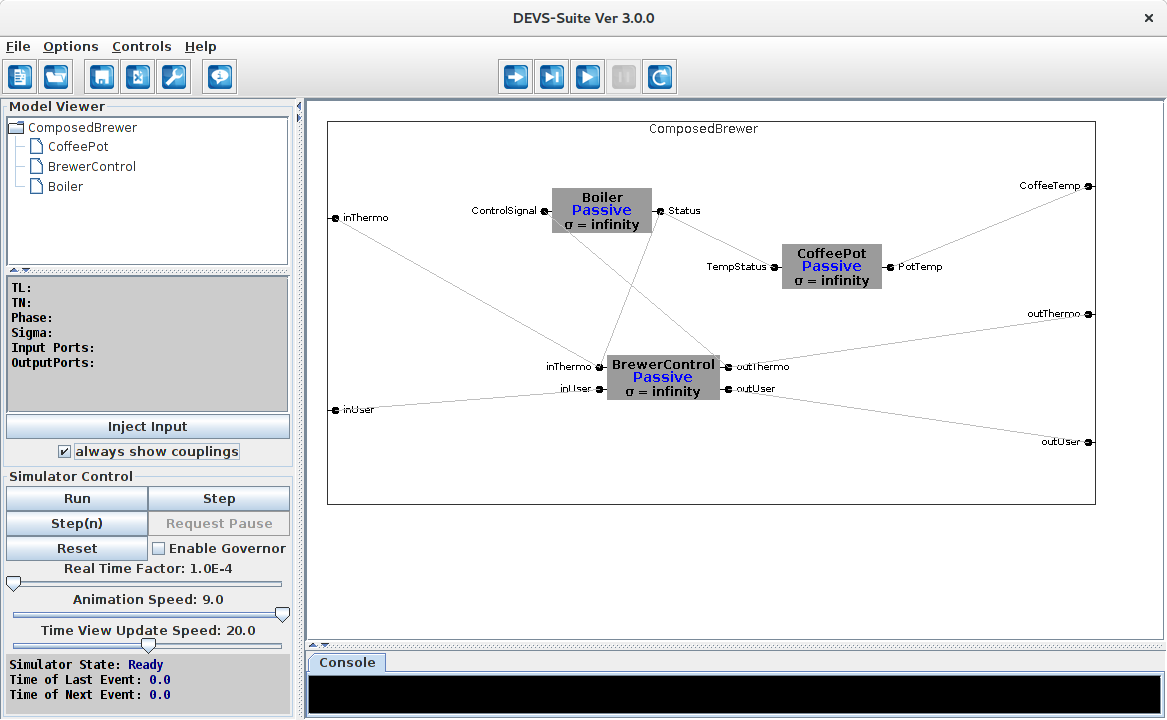
\includegraphics[width=0.8\textwidth]{input/model-in-devs}
      \caption{Coffee Brewer Coupled Model Within DEVS Suite Simulator}
      \label{ref:modInDevs}
    \end{center}
  \end{figure}
\end{center}

This project employs a sequential approach to simulation execution.  While the premise of a parallel and/or distributed strategy seems attractive, the scope of the project, low anticipated computational demand of the simulation, and availability of high performance computers suggest that a parallel/distributed strategy does not meet the cost-benefit threshold.  That said, the distinction between model and simulator in the project documentation and code provides a foundation for further extension of the project (outside of the scope of the course) into the realm of distributed simulation models.

\subsubsection{Experimental Frame}
The experimental frame for any simulation captures the lens for the experimentation and is a key component of simulation strategy.  By building Requester and Transducer models, the experimental frame can be formalized.  For this project, user inputs and artificial thermocouple readings are the most important means to stimulate the model.  As such, these capabilities are built into the Requester model.  The most important metric for discerning coffee quality is the temperature of the coffee pot.  With this in mind, the Transducer is integrated into the model and coupled in order to record this important value.

\begin{center}
  \begin{figure}[H]
    \begin{center}
      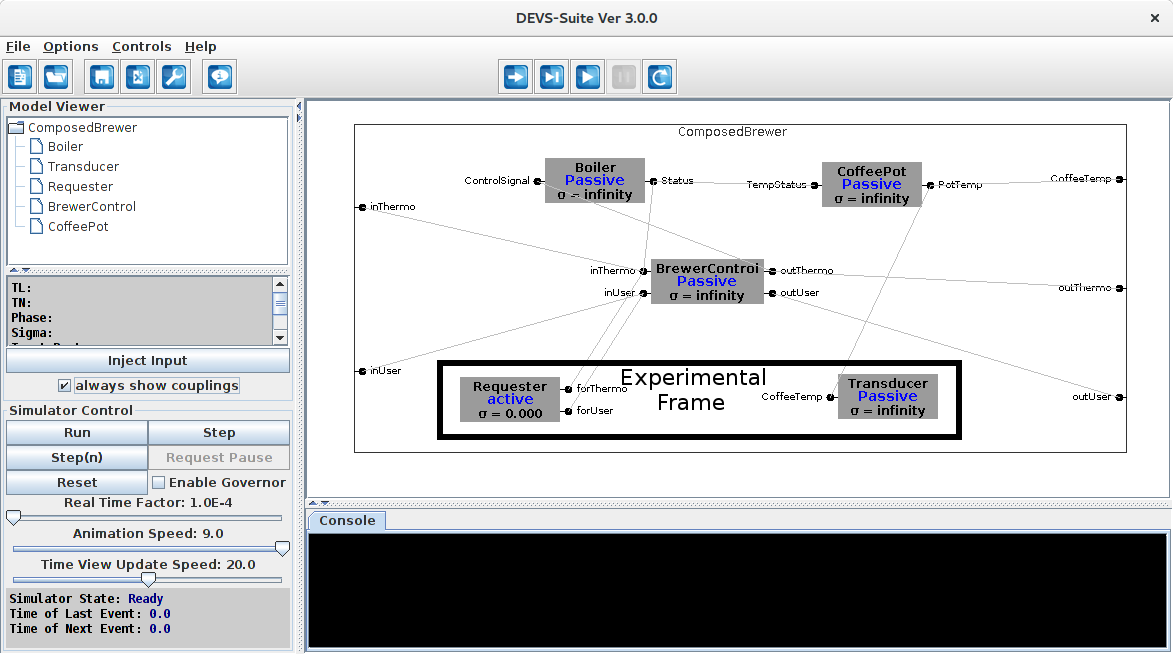
\includegraphics[width=0.8\textwidth]{input/ef-introduced}
      \caption{Experimental Frame Built Into Model}
      \label{ref:ef-introduced}
    \end{center}
  \end{figure}
\end{center}


\subsubsection{Animation}
An important aspect of simulation strategy is the approach to interpreting simulation results.  Seeing as the coffee brewer system has an intuitive and natural physical representation, animation is of substantial value.  While this provides no new data, it does provide more in the way of insights/value.  Additionally, animation enables a wider audience, particularly those with a non-technical background, to understand and interpret results.

For this project animation was implemented using a separate program, developed from scratch in Python.  During execution, the DEVS system was programmed to output key value pairs to regular system files within the project directory.  The Python animation program is started separately from the DEVS simulation.  Through a continuous refresh, the Python animation can track the progress of the DEVS simulation as the user ``steps'' through the model execution.  A screenshot of the animation program is provided below.

\begin{center}
  \begin{figure}[H]
    \begin{center}
      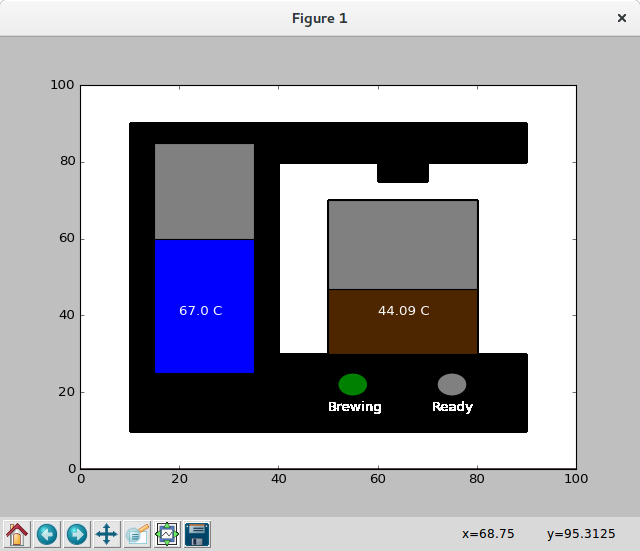
\includegraphics[width=0.6\textwidth]{input/animation}
      \caption{Coffee Brewer Animation}
      \label{ref:cofBreAni}
    \end{center}
  \end{figure}
\end{center}


\subsection{Experimental Details}
The modeling and simulation of the coffee maker was primarily focused on more quantitative safety and functional features. This included the safety shutoff feature, the overheat prevention shutoff, and the temperature of the coffee. Tests were conducted using variation in heat flux and vertical flow. The temperature within the boiler and coffee pot was collected at each time interval. The difference between those temperatures at different heat flux values will be compared, along with whether or not a particular shut down mechanism was activated.

\subsubsection{Regular Brew}
\begin{multicols}{2}
Boiler Setup
\begin{itemize}
\item TimeStep = 1 $sec$
\item HeatFlux = 900 $W$
\item Volume = 0.001 $m^3$ (1 Liter)
\item Density = 1000 $\frac{kg}{m^3}$
\item HeatCapacity = 4180 $\frac{J}{kg*C}$
\item Flow = 240 $sec$ (to fill pot)
\end{itemize}

\columnbreak
Controller Setup
\begin{itemize}
\item RegistrationTime = 1.5 $sec$ (User Input Latency)
\item SafetyTimeout = 600 $sec$
\item DisplayTime = 0.5 $sec$ (User Output Latency)
\item IndicatorTimeout = 300 $sec$
\item MaxSafeTemp = 100 $degrees~Celsius$
\end{itemize}

\end{multicols}

\begin{center}
  \begin{figure}[H]
    \begin{subfigure}{.5\textwidth}
      \centering
      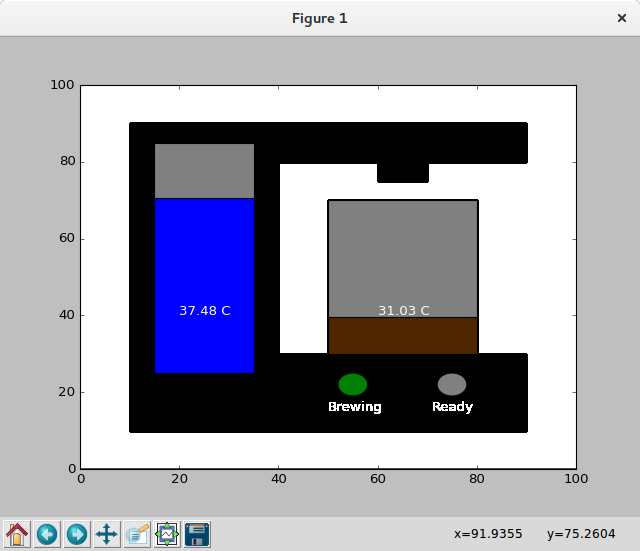
\includegraphics[width=.8\linewidth]{input/test-1-prog}
      \caption{Coffee Maker After One Minute}
      \label{fig:test-1-prog}
    \end{subfigure}%
    \begin{subfigure}{.5\textwidth}
      \centering
      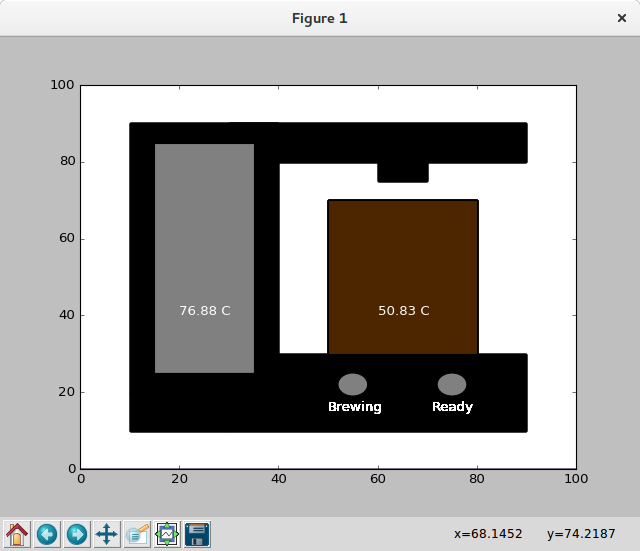
\includegraphics[width=.8\linewidth]{input/test-1}
      \caption{Coffee Maker End State}
      \label{fig:test-1}
    \end{subfigure}
  \caption{Regular Brew Status Snapshots}
  \end{figure}
\end{center}
\begin{center}
  \begin{figure}[H]
    \begin{center}
      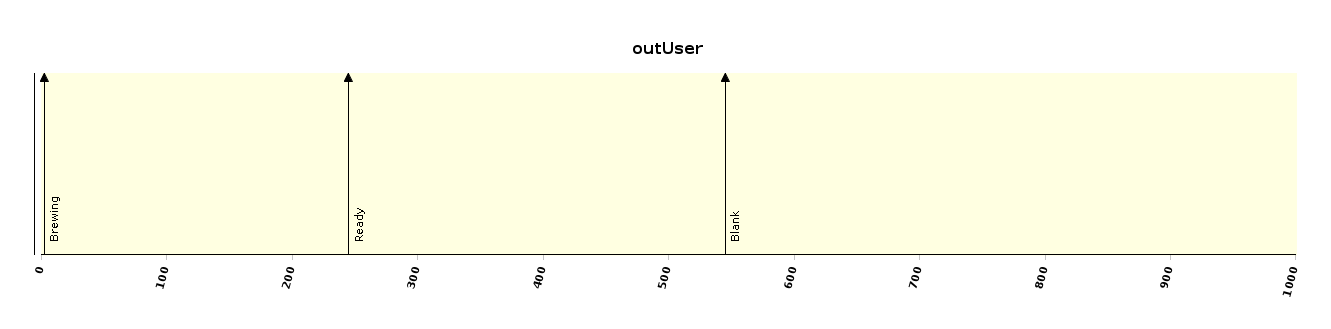
\includegraphics[width=0.6\textwidth]{input/test-1-plot}
      \caption{User Indicator Progression}
      \label{ref:test-1-plot}
    \end{center}
  \end{figure}
\end{center}


\subsubsection{Safety Timeout}
\begin{multicols}{2}
Boiler Setup
\begin{itemize}
\item TimeStep = 1 $sec$
\item HeatFlux = 300 $W$
\item Volume = 0.001 $m^3$ (1 Liter)
\item Density = 1000 $\frac{kg}{m^3}$
\item HeatCapacity = 4180 $\frac{J}{kg*C}$
\item Flow = 900 $sec$ (to fill pot)
\end{itemize}

\columnbreak
Controller Setup
\begin{itemize}
\item RegistrationTime = 1.5 $sec$ (User Input Latency)
\item SafetyTimeout = 600 $sec$
\item DisplayTime = 0.5 $sec$ (User Output Latency)
\item IndicatorTimeout = 300 $sec$
\item MaxSafeTemp = 100 $degrees~Celsius$
\end{itemize}

\end{multicols}

\begin{center}
  \begin{figure}[H]
    \begin{subfigure}{.5\textwidth}
      \centering
      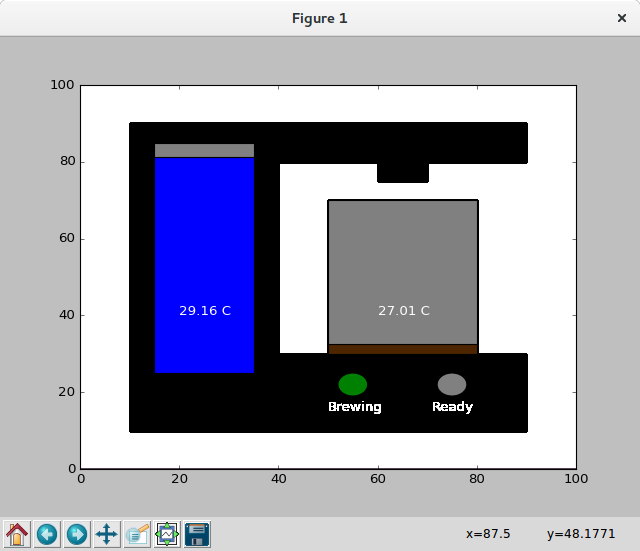
\includegraphics[width=.8\linewidth]{input/test-2-prog}
      \caption{Coffee Maker After One Minute}
      \label{fig:test-2-prog}
    \end{subfigure}%
    \begin{subfigure}{.5\textwidth}
      \centering
      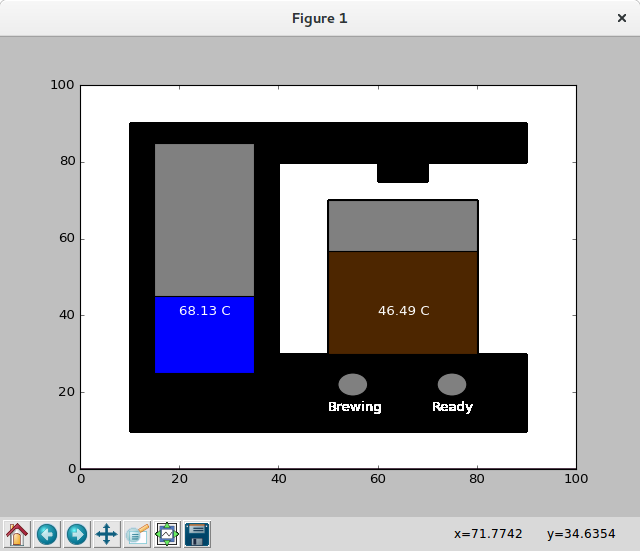
\includegraphics[width=.8\linewidth]{input/test-2}
      \caption{Coffee Maker End State}
      \label{fig:test-2}
    \end{subfigure}
  \caption{Safety Timeout Status Snapshots}
  \end{figure}
\end{center}
\begin{center}
  \begin{figure}[H]
    \begin{center}
      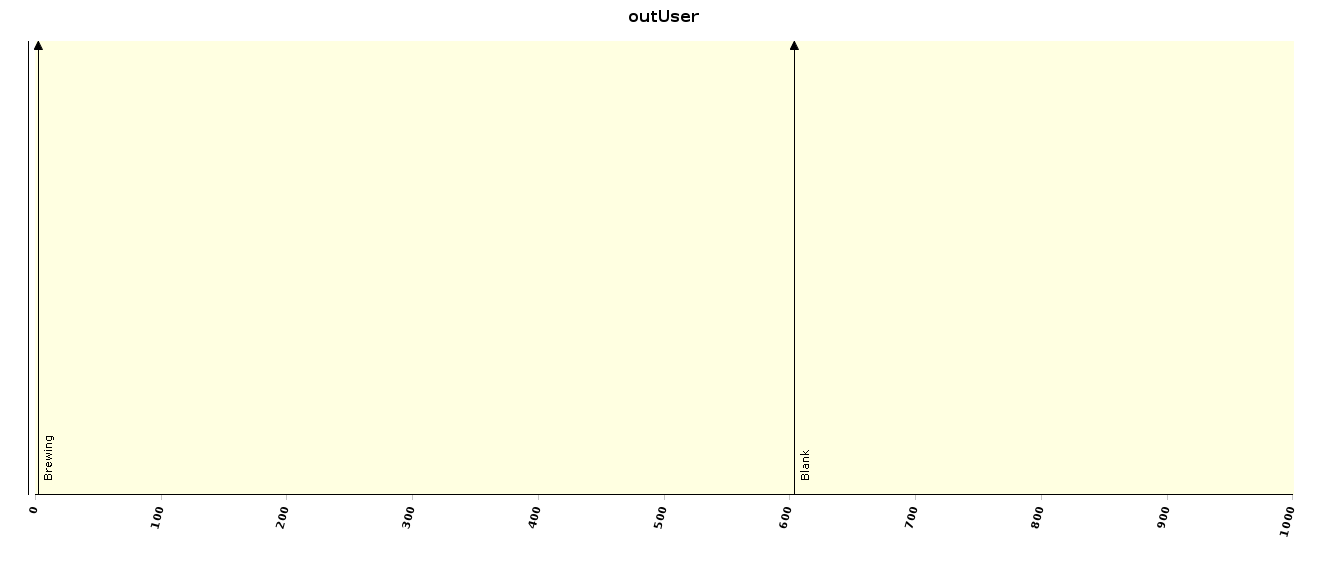
\includegraphics[width=0.6\textwidth]{input/test-2-plot}
      \caption{User Indicator Progression}
      \label{ref:test-2-plot}
    \end{center}
  \end{figure}
\end{center}


\subsubsection{Overheat Shutoff}
\begin{multicols}{2}
Boiler Setup
\begin{itemize}
\item TimeStep = 1 $sec$
\item HeatFlux = 800 $W$
\item Volume = 0.001 $m^3$ (1 Liter)
\item Density = 1000 $\frac{kg}{m^3}$
\item HeatCapacity = 4180 $\frac{J}{kg*C}$
\item Flow = 800 $sec$ (to fill pot)
\end{itemize}

\columnbreak
Controller Setup
\begin{itemize}
\item RegistrationTime = 1.5 $sec$ (User Input Latency)
\item SafetyTimeout = 600 $sec$
\item DisplayTime = 0.5 $sec$ (User Output Latency)
\item IndicatorTimeout = 300 $sec$
\item MaxSafeTemp = 100 $degrees~Celsius$
\end{itemize}

\end{multicols}

\begin{center}
  \begin{figure}[H]
    \begin{subfigure}{.5\textwidth}
      \centering
      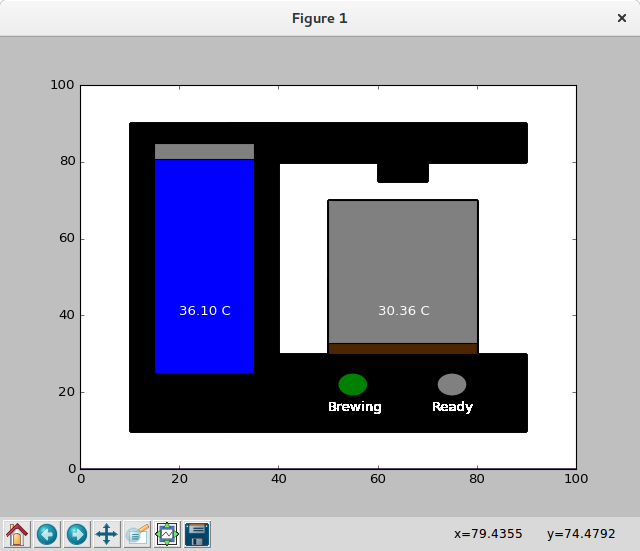
\includegraphics[width=.8\linewidth]{input/test-3-prog}
      \caption{Coffee Maker After One Minute}
      \label{fig:test-3-prog}
    \end{subfigure}%
    \begin{subfigure}{.5\textwidth}
      \centering
      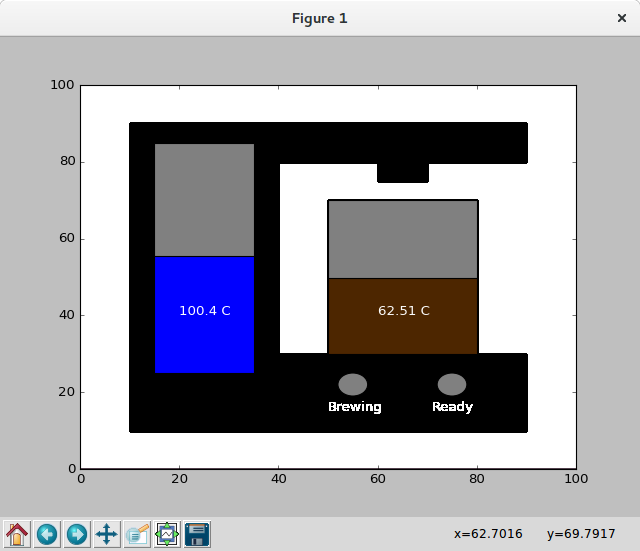
\includegraphics[width=.8\linewidth]{input/test-3}
      \caption{Coffee Maker End State}
      \label{fig:test-3}
    \end{subfigure}
  \caption{Overheat Shutoff Status Snapshots}
  \end{figure}
\end{center}
\begin{center}
  \begin{figure}[H]
    \begin{center}
      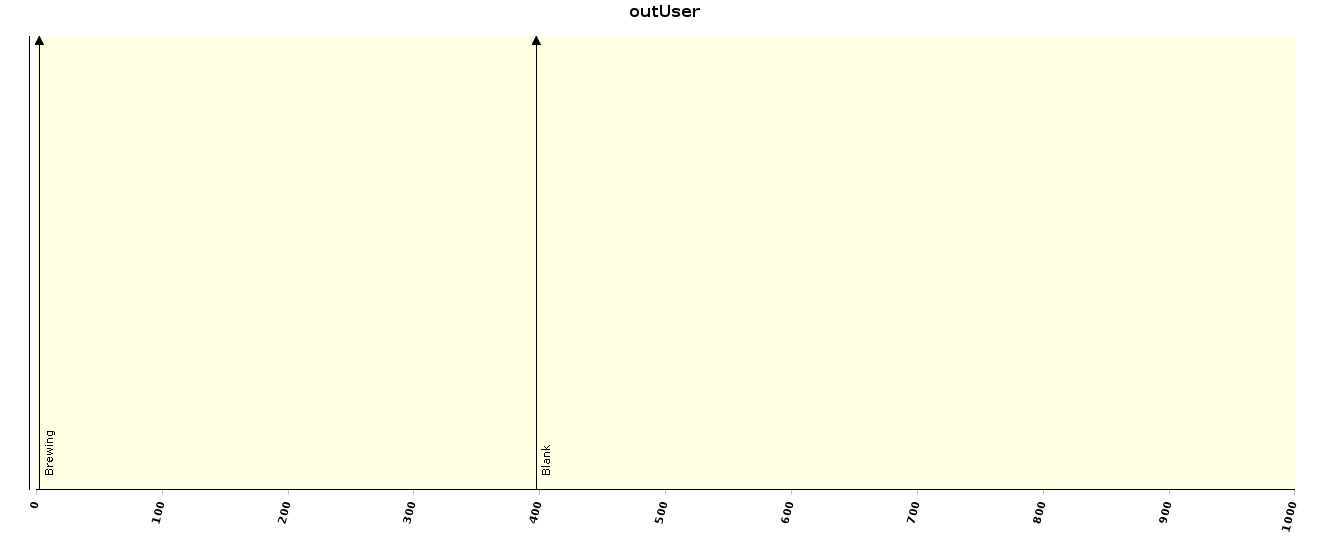
\includegraphics[width=0.6\textwidth]{input/test-3-plot}
      \caption{User Indicator Progression}
      \label{ref:test-3-plot}
    \end{center}
  \end{figure}
\end{center}

%% ~\\
%% Some additional tests include:
%% \begin{center}
%%   \begin{tabular}{| p{2.5cm} | p{3.3cm} | p{3.3cm} | p{3.3cm} | p{2.5cm} |} \hline
%% \textbf{Test Cases} &
%% \textbf{Time Frame} &
%% \textbf{Boiler Empty?} &
%% \textbf{Expected Output} &
%% \textbf{Result} \\ \hline \hline
%% Test Case 1.0 &
%% 2 min &
%% False &
%% $<$ 205$^{\circ}$ &
%% TBD \\ \hline
%% Test Case 1.1 &
%% 2 min &
%% True &
%% Safety Shut Off &
%% TBD \\ \hline
%% Test Case 2.0 &
%% 4 min &
%% False &
%% $\approx$ 205$^{\circ}$ &
%% TBD \\ \hline
%% Test Case 2.1 &
%% 4 min &
%% True &
%% Safety Shut Off &
%% TBD \\ \hline
%% Test Case 3.0 &
%% 6 min &
%% False &
%% $>$ 205$^{\circ}$ &
%% TBD \\ \hline
%% Test Case 3.1 &
%% 6 min &
%% True &
%% Safety Shut Off &
%% TBD \\ \hline
%% Test Case 4.0 &
%% 20 min &
%% False &
%% Safety Shut Off &
%% TBD \\ \hline
%% Test Case 4.1 &
%% 20 min &
%% True &
%% Safety Shut Off &
%% TBD \\ \hline
%% \end{tabular}
%% \end{center}

\section{Results}
The simulation was run under the regular brew, safety timeout, and overheat shutoff settings. In
the regular brew settings, the temperature of the output coffee was below the safety threshold and was
lower that what would typically be expected for coffee by about $20^o$C, sitting at $50^o$C. Under the safety
timeout settings, the coffee does not completely brew. About 2/3 of the pot is brewed in 10
minutes before the shutoff occurs. In the overheat shutoff test, the boiler had exceeded the
acceptable safety threshold temperature within 6 minutes. This also made it impossible to complete the
pot.

There is some evidence of strong results verification for the simulation runs.  For example, the emergency timeout occurs right at the expected 10 minute mark during that simulation run.  Further, the temperature barely reaches $100^o$C during the overheat shutoff case and the brew time matches expectation in the baseline simulation.  The simulator and modeling approach have been successfully adapted to a wide variety of projects, which provides some additional confidence with respect to verification.  Validation on the other hand is a more difficult assessment.  The timing and temperatures for the coffee brewing are within a physically intuitive range.  However, structuring the system so that the pump and heating element always operate together appears to generate some behavior that doesn't align with real world experience.  It may be preferable to model the system in such a way that the pump does not operate until the water is at a sufficiently high temperature.  Independent operation of the pump and heating element is an option for future exploration and an approach which is likely to result in better model validation.


\section{Conclusions}
There is an intuitive relationship between the heat flux, fluid flow rate, and the coffee brewers ability to
complete the pot without exceeding temperature and time limits. Particularly, even with a
relatively low heat flux, a low volumetric flow will result in the brewer shutting down before filling the
pot. It makes logical sense for a low rate of transfer from the boiler to delay the brewing beyond a
reasonable time frame. What would be worthy of examination in the future would be the use of a higher
volumetric flow in order to manage a greater heat flux. This may prevent overheating while
allowing the pot to fill. There would likely be an increase in the speed in which it fills as well. Therefore, it
would be beneficial to look further into the degree of heat flux allowed in relation to volumetric flow.

\newpage
\section{References}
\doublespace
\hin Coffee market ends 2016/17 coffee year in deficit for the third consecutive year. (2017, July 31). Retrieved October 16, 2017, from http://www.ico.org/prices/po-production.pdf

\hin Frei, G. (2016, April 11). Gewicht und Grösse der Elefanten. Retrieved October 16, 2017, from https://de.upali.ch/gewicht-und-grosse/

\hin Ptolemaeus, C. (2014). System design, modeling, and simulation: using Ptolemy II. Berkeley: Ptolemy.org.

\hin Sarjoughian, H. (2017). Chapter 1 - Modeling Concepts WorldView Applications [Powerpoint slides]. Retrieved from https://myasucourses.asu.edu/bbcswebdav/pid-16267679-dt-content-rid-105794536\_1/xid-105794536\_1

\hin Sarjoughian, H. S., \& Sundaramoorthi, S. (2015, April). Superdense time trajectories for DEVS simulation models. In Proceedings of the Symposium on Theory of Modeling \& Simulation: DEVS Integrative M\&S Symposium (pp. 249-256). Society for Computer Simulation International.

\hin Zeigler, B. P., Kim, T. G., \& Praehofer, H. (2010). Theory of modeling and simulation: integrating discrete event and continuous complex dynamic systems. Amsterdam: Acad. Press
\singlespace

\newpage
\section{Appendices}
\subsection{Appendix A - ComposedBrewer Model}
\begin{scriptsize}
\lstinputlisting[language=Java]{../../devs-coffee-brewin/DEVS_Suite_3.0.0_executable_linux_64/src/CoffeeBrewin/ComposedBrewer.java}
\end{scriptsize}
\newpage
\subsection{Appendix B - Pot Model}
\begin{scriptsize}
\lstinputlisting[language=Java]{../../devs-coffee-brewin/DEVS_Suite_3.0.0_executable_linux_64/src/CoffeeBrewin/Pot.java}
\end{scriptsize}
\newpage
\subsection{Appendix C - Boiler Model}
\begin{scriptsize}
\lstinputlisting[language=Java]{../../devs-coffee-brewin/DEVS_Suite_3.0.0_executable_linux_64/src/CoffeeBrewin/Boiler.java}
\end{scriptsize}
\newpage
\subsection{Appendix D - BrewerControl Model}
\begin{scriptsize}
\lstinputlisting[language=Java]{../../devs-coffee-brewin/DEVS_Suite_3.0.0_executable_linux_64/src/CoffeeBrewin/BrewerControl.java}
\end{scriptsize}
\newpage
\subsection{Appendix E - Requester Model}
\begin{scriptsize}
\lstinputlisting[language=Java]{../../devs-coffee-brewin/DEVS_Suite_3.0.0_executable_linux_64/src/CoffeeBrewin/Requester.java}
\end{scriptsize}
\newpage
\subsection{Appendix F - Transducer Model}
\begin{scriptsize}
\lstinputlisting[language=Java]{../../devs-coffee-brewin/DEVS_Suite_3.0.0_executable_linux_64/src/CoffeeBrewin/Transducer.java}
\end{scriptsize}
\newpage
\subsection{Appendix G - Animator Code}
\begin{scriptsize}
\lstinputlisting[language=Python]{../../devs-coffee-brewin/DEVS_Suite_3.0.0_executable_linux_64/py/plot-along.py}
\end{scriptsize}



\end{document}
